%\chapter{T-Ringの設計実装}
\chapter{設計と実装}
\begin{large}
\begin{quote}
本章では,T-Ringにおける詳細な設計,実装について解説する.
\end{quote}
\end{large}
\clearpage

\section{システム構成}
本節では,T-Ringシステムの設計について述べる.T-Ringを構成する保存ピアはネットワークモジュール,センサ情報管理モジュール,データ保存モジュール,データ取得モジュール,保存ピア発見モジュール,センサ管理モジュール,アプリケーションモジュールの7つのモジュールによって構成される.図\ref{fig:sysconf}がシステム構成図であり,各モジュール間でのデータの受け渡しが記述されている.

\begin{figure}[htbp]
 \begin{center}
  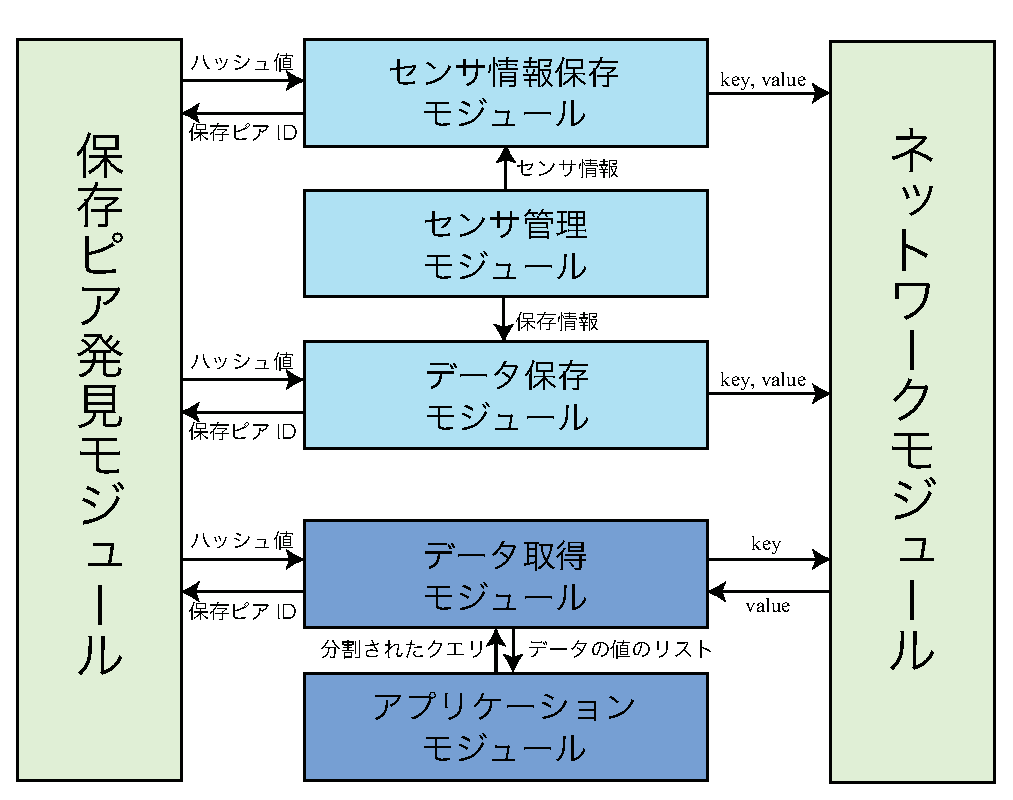
\includegraphics[width=130mm]{./images/sysconf.eps}
 \end{center}
 \caption{システム構成図}
 \label{fig:sysconf}
\end{figure}

%\subsection{ネットワークモジュール}
%ネットワークモジュールは保存ピア同士で協調し,1Dトーラス型のオーバーレイネットワークを構築及びデータに関する通信を行うモジュールである.本モジュールでは,他の保存ピアのデータ取得モジュールから,データ取得のクエリが送られた場合に,対象のデータをクエリ送信元の保存ピアに送信する.
%
%本モジュールの実装はオープンソースであるOpenChordの一部を参考にしている.保存ピアのJoin,Retrieveなどの保存ピアによるネットワークの構築の部分において利用している.
%
%\subsection{センサ情報管理モジュール}
%本モジュールは,センサの緯度や経度など,センサデータの値以外の多次元データとしてのセンサ情報を適切な場所に保存することで,データの取得を可能にするモジュールである.
%
%センサデータの取得を考えた際に,一般的な手法は,センサノードのアドレスを指定して取得するが,T-Ringが想定している環境では,センサデータをアドレス以外の他の要素から取得する.よって,取得を行う時には,取得されるセンサデータの情報が必要である.このために,T-Ringでは,対象のセンサノードの緯度,経度,センサタイプ,マスターピア=0で一次元化,ハッシュ化した値を担当する保存ピアに対して,このセンサ情報を登録する.登録はセンサデータの値の保存と同様に行う.センサデータの保存については,次節で詳細に述べる.保存におけるキーとして,緯度,経度,センサタイプ,マスターピア=0の4次元値を1次元化,ハッシュ化した値を,バリューとして,そのセンサのchunkとSPの時間のセットを保存する.データの取得については,5.4で詳細に述べるが,データの取得の際には,緯度,経度,センサタイプ,chunk,SPの時間を必要とする.緯度,経度,センサタイプ,マスターピア=0の担当ピアに取得に必要なセンサ情報を登録することによって,chunkとSPの時間を知ることが可能になる.
%
%本モジュールでは,最初に,センサに関する情報が登録されているSensorInfo.csvから,センサIDをキーとして,センサデータの保存に必要である,緯度,経度,センサタイプ,chunk,SPの時間を取得する.取得された情報から,緯度,経度,センサタイプ,マスターピア=0の4次元値をZ-order関数によって処理し,返されたバイナリ値を保存ピア発見モジュールに渡す.保存ピア発見モジュールは,担当の保存ピアの保存ピアIDを返してくるので,そのピアに対して必要な情報を登録する.
%\if0
%\begin{lstlisting}[caption=センサ情報の登録]
%
%public class StoreSensorInformationThread extends Thread {
%	private String sensorId;
%	private String fileName;
%	private String tmpName;
%	private FileProcessor fileProcessor;
%	private File tmp;
%	private InformationDeliveryInterface informationDelivery;
%
%	public StoreSensorInformationThread(JoinData joinData, String id) {
%		this.sensorId = id;
%		this.fileName = "sensorInfo.csv";
%		this.tmpName = "sensorInfo.tmp";
%		this.fileProcessor = new FileProcessor(fileName, tmpName);
%		this.tmp = new File(tmpName);
%		this.informationDelivery = new InformationDeliveryImpl(joinData);
%	}
%	
%	public void run(){
%		SensorInformation sensorInformation = new SensorInformation();
%		
%		long getLineNum = 0;
%		getLineNum = fileProcessor.searchLine(sensorId, tmp);
%		
%		String[] sensorInfoList = null;
%		
%		sensorInfoList = fileProcessor.getLine(getLineNum);
%		
%		if (sensorInfoList != null) {
%			for (int i = 0; i < sensorInfoList.length; i++) {
%				switch(i){
%				case 1:
%					long latitude = Long.parseLong(sensorInfoList[i]);
%					sensorInformation.latitude = latitude;
%					break;
%				case 2:
%					long longitude = Long.parseLong(sensorInfoList[i]);
%					sensorInformation.longitude = longitude;
%					break;
%				case 3:
%					long sensorType = Long.parseLong(sensorInfoList[i]);
%					sensorInformation.type = sensorType;
%					break;
%				case 4:
%					long chunkTime = Long.parseLong(sensorInfoList[i]);
%					sensorInformation.chunk = chunkTime;
%					break;
%				case 5:
%					long startPointTime = Long.parseLong(sensorInfoList[i]);
%					sensorInformation.startPoint = startPointTime;
%					break;
%				case 7:
%					long configTime = Long.parseLong(sensorInfoList[i]);
%					sensorInformation.configTime = configTime;
%					break;
%				}
%			}
%		} else {
%			System.out.println(sensorId + " isn't in " + fileName);
%		}
%		informationDelivery.storeSensorInformation(sensorInformation);
%	}
%}
%\end{lstlisting}
%\fi
%\subsection{データ保存モジュール}
%本モジュールはセンサデータを保存する保存するモジュールである.
%
%T-Ringでは,センサデータの時間に従って保存先を決めるため,センサ管理モジュールから,センサID,対象データの緯度,経度,センサタイプ,chunk,SPの時間,データの時間,センサの設定時間を取得する.本モジュールでは,フィールドとして,センサIDをキーに,次に保存すべき保存ピアのIDをバリューとするMapを所持している.送られてきたセンサIDとMap内のセンサIDを比較し,登録されていない場合は,データの時間,センサの設定時間,chunkから,まず,マスターピアの番号を決定する.次いで,そのマスターピアからSuccessorを辿る回数を計算する.そして,緯度,経度,センサタイプ,マスターピアの番号の4次元からハッシュ化をし,その値とSuccessorを辿る回数を保存ピア発見モジュールに送る.その結果として保存ピアIDを受け取る.データが保存されるセンサのIDとMap内のセンサIDが一致していた場合は,そのMapのセンサIDに対応する保存ピアのIDを取得する.次に,そのIDの保存ピアに対して,キーを緯度,経度,センサタイプの1次元化とハッシュ値,バリューをデータの値として保存する.
%
%また,保存が行われると,次に保存するべき保存ピアの計算が行われる.ここからはセンサのIDとデータの時間だけを監視する.この計算を行うために,センサIDをキーとして,最新のセンサデータが保存された保存ピアのID,マスターピアの番号それぞれをバリューとして保存する2つのフィールドが存在する.次に送られてきたデータが前回のデータと比較してchunkが異なっていた場合,保存ピア発見モジュールに対して,最新の保存データが保存された保存ピアIDとSuccessorを辿る回数が送られる.これに対して,対象の保存ピアのIDが返される.この保存ピアのIDを次に保存すべき保存ピアIDとして更新する.次に,chunkが同一であった場合,最新の保存データが保存された保存ピアIDを次に保存すべき保存ピアIDをとして更新する.マスターピアが異なっていた場合,センサIDが登録されていない時と同様の処理を行い,保存ピア発見モジュールから返された保存ピアIDを次に保存すべき保存ピアIDとして更新する.
%
%これらの処理が繰り返えされることにより,データの保存が行われる.以上に述べた処理をフローチャートで示す.
%
%\subsection{データ取得モジュール}
%アプリケーションモジュールから送られるユーザからの取得のクエリは,範囲を持ったクエリであるので,本モジュールにより,クエリの緯度,経度,半径から分割を行う.これについては図\ref{fig:divide}が例と図解である.そして,分割を行ったそれぞれの位置について,緯度,経度,センサタイプとクエリで指定された取得時間から,データ保存と同じ手順により,緯度,経度,センサタイプ,マスターピアの番号の4次元によるハッシュ値,Successorを辿る回数を保存ピア発見モジュールに送り,その結果として受け取った保存ピアIDに対して,緯度,経度,センサタイプで生成されるキーからバリューを受け取る.この受け取ったバリューのセットを,指定された方式に変換しアプリケーションモジュールに送り返す.指定された方式に関しては,アプリケーションモジュールの解説の際に説明する.
%
%\begin{figure}[htbp]
% \begin{center}
%  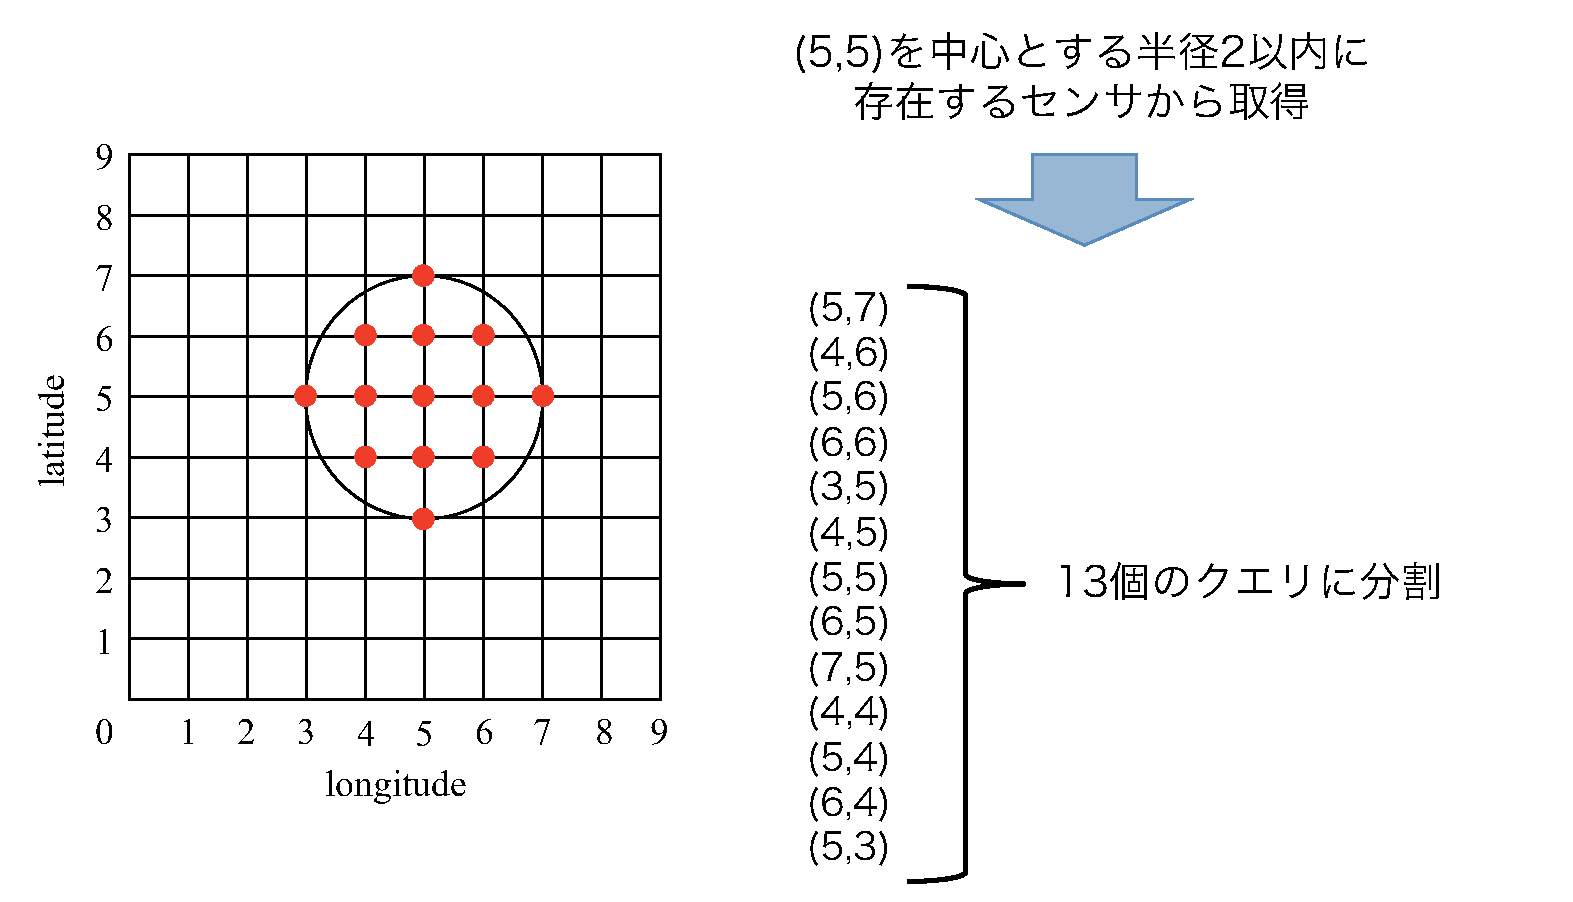
\includegraphics[width=130mm]{./images/divide.eps}
% \end{center}
% \caption{クエリの分割}
% \label{fig:divide}
%\end{figure}
%
%\subsection{保存ピア発見モジュール}
%本モジュールは,センサ情報管理モジュール,データ保存モジュール,データ取得モジュールから受け取ったハッシュ値やSuccessorを辿る回数から,対象の保存ピアを発見し,そのアドレスを各モジュールに送り返す.
%
%T-Ringでは2種類の保存ピアの発見の方法が存在する,1つ目は,Finger Tableを用いた発見である.Finger Tableの計算回数は$O(\log{2}N)$である.この発見はデータ保存モジュール,データ取得モジュールから送られた緯度,経度,センサタイプ,マスターピアの番号の4次元によるハッシュ値が前データと異なる場合に,マスターピアを探索するために行われる.また,Synapseにおける保存,取得では,センサデータ毎にこの計算がなされる.
%
%2つ目の方法は,データ保存モジュール,データ取得モジュールから送られた緯度,経度,センサタイプ,マスターピアの番号の4次元によるハッシュ値が前データと同様であった場合に行われる.この場合,前データで取得したアドレスのSuccessorのアドレスを取得する.Finger Tableによる計算は前データの際に行ったため,計算回数は$O(1)$である.
%
%これらの方法により発見されたアドレスをデータ保存モジュール,データ取得モジュールに送り返す.
%
%\begin{lstlisting}[caption=データ保存時の保存ピア発見]
%public class NextStorePeer {
%	private TRingImpl tring;
%	private HashMap<String, Node> nextNode;
%	private HashMap<String, Long> restTime;
%	private HashMap<String, Long> prevSP;
%	private HashMap<String, Long> prevTime;
%	ArrayList<Long> positions;
%
%	public NextStorePeer(JoinData joinData) {
%		this.positions = new ArrayList<Long>();
%		this.nextNode = new HashMap<String, Node>();
%		this.restTime = new HashMap<String, Long>();
%		this.prevSP = new HashMap<String, Long>();
%		this.prevTime = new HashMap<String, Long>();
%		this.tring = joinData.tring;
%	}
%
%	public synchronized Node getNextStorePeer(Node node, DataForStore data,
%			Key key) throws CommunicationException {
%		setNextStorePeer(node, data, key);
%		return nextNode.get(Arrays.toString(key.getBytes()));
%	}
%
%	private synchronized void setNextStorePeer(Node currentPeer,
%			DataForStore data, Key key) throws CommunicationException {
%		long SP = (data.time - data.configTime) / data.startPoint;
%
%		if (nextNode.get(Arrays.toString(key.getBytes())) == null) {
%			this.nextNode
%					.put(Arrays.toString(key.getBytes()), currentPeer
%							.findSuccessor(currentPeer.getNodeAddingOneID()));
%			this.prevSP.put(Arrays.toString(key.getBytes()), SP);
%			this.restTime.put(Arrays.toString(key.getBytes()), data.startPoint
%					- data.chunk);
%		} else {
%			if (this.prevSP.get(Arrays.toString(key.getBytes())) != SP) {
%				this.positions.add(data.latitude);
%				positions.add(data.longitude);
%				positions.add(data.type);
%				this.positions.add(SP);
%				ZorderInterface zorder = new Zorder(positions);
%				byte[] SPKey = zorder.getZorder();
%				Key masterPeerKey = new ByteArrayKey(SPKey);
%				nextNode.put(Arrays.toString(key.getBytes()),
%						tring.getResponsiblePeer(masterPeerKey));
%				this.prevSP.put(Arrays.toString(key.getBytes()), SP);
%			} else if (restTime.get(Arrays.toString(key.getBytes()))
%					- data.chunk > 0) {
%				this.nextNode.put(Arrays.toString(key.getBytes()), currentPeer
%						.findSuccessor(currentPeer.getNodeAddingOneID()));
%			}
%			this.restTime.put(Arrays.toString(key.getBytes()), data.startPoint
%					- data.chunk);
%		}
%	}
%}
%\end{lstlisting}
%
%\begin{lstlisting}[caption=データ取得時の保存ピア発見]
%
%public class NextRetrievePeer {
%	private TRingImpl tring;
%	private HashMap<String, Node> nextNode;
%	private HashMap<String, Long> restTime;
%	private HashMap<String, Long> prevSP;
%	ArrayList<Long> retrievedData;
%	ArrayList<Long> positions;
%
%	public NextRetrievePeer(TRingImpl tring) {
%		this.positions = new ArrayList<Long>();
%		this.nextNode = new HashMap<String, Node>();
%		this.restTime = new HashMap<String, Long>();
%		this.prevSP = new HashMap<String, Long>();
%		this.retrievedData = new ArrayList<Long>();
%		this.tring = tring;
%	}
%
%	public synchronized ArrayList<Long> getNextRetrievePeer(
%		DataForRetrieve data, long latitude, long longitude,
%		HashMap<String, Long> sensorInfo, Key key)
%		setNextRetrievePeer(data, latitude, longitude, sensorInfo, key);
%		return this.retrievedData;
%	}
%
%	private synchronized void setNextRetrievePeer(DataForRetrieve data,
%			long latitude, long longitude, HashMap<String, Long> sensorInfo,
%			Key key) throws CommunicationException {
%		String tag = Arrays.toString(key.getBytes());
%		long currentTime = data.timeFrom;
%		long SPTime = sensorInfo.get("SP");
%		long chunk = sensorInfo.get("chunk");
%		long configTime = sensorInfo.get("configTime");
%		long SP = (currentTime - configTime) / SPTime;
%		long pastTime = currentTime - configTime - (SP * SPTime);
%		long leftChangeTime = SPTime - pastTime;
%		long leftTime = data.timeTo - currentTime;
%
%		ArrayList<Long> positions = new ArrayList<Long>();
%		positions.add(latitude);
%		positions.add(longitude);
%		positions.add(data.type);
%		positions.add(SP);
%		ZorderInterface zorder = new Zorder(positions);
%		byte[] SPKey = zorder.getZorder();
%		Key masterPeerKey = new ByteArrayKey(SPKey);
%
%		nextNode.put(tag, tring.getResponsiblePeer(masterPeerKey));
%
%		Node currentNode = nextNode.get(tag);
%
%		while (leftTime > 0) {
%			leftTime -= chunk;
%			leftChangeTime -= chunk;
%
%			if (leftChangeTime > 0) {
%				this.retrievedData.addAll(tring.retrieveData(key,
%						this.nextNode.get(tag)));
%				this.nextNode.put(
%						tag,
%						this.nextNode.get(tag).findSuccessor(
%				this.nextNode.get(tag).getNodeAddingOneID()));
%				
%			} else {
%				leftChangeTime += SPTime;
%				positions.set(3, positions.get(3) + 1);
%				zorder = new Zorder(positions);
%				SPKey = zorder.getZorder();
%				masterPeerKey = newByteArrayKey(SPKey);
%				this.nextNode.put(tag,this.nextNode.get(tag).findSuccessor(this.nextNode.get(tag).getNodeAddingOneID()));	
%				this.retrievedData.addAll(tring.retrieveData(key,this.nextNode.get(tag)));
%				
%			}
%		}
%	}
%}
%\end{lstlisting}
%
%\subsection{センサ管理モジュール}
%本モジュールはセンサネットワーク内のセンサ毎の緯度,経度,センサタイプ,などを管理を行うモジュールである.センサが環境に設置された際に,そのセンサの情報を所属する保存ピアへ登録する.また,センサの移動により,緯度,経度の変更が発生した際に,その情報を更新する.
%
%センサが環境に設置を行う際,以下のようなセンサ情報登録クラスのインスタンスを用いてSensorInfo.csvに登録を行う.SensorInfo.csvに登録されるエントリは,各センサごとに,sensorId,latitude,longitude,sensorType,chunkTime,startPointTimeである.センサの設置場所が変更された際は,sensorIdから対象のエントリを発見し,変更を行う.このSensorInfo.csvの情報は,センサ情報保存モジュール,データ保存モジュールで利用される.以下がセンサ情報の登録,変更のメインクラスである.
%\if0
%\begin{lstlisting}[caption=センサ情報の保存,変更]
%
%public class SensorInfo {
%	private String fileName;
%	private String tmpName;
%	private FileProcessor fileProcessor;
%	private int num;
%	
%	public SensorInfo(String fileName, String tmpName) {
%		this.fileName = fileName;
%		this.tmpName = tmpName;
%		this.fileProcessor = new FileProcessor(fileName, tmpName);
%		this.num = 0;
%	}
%
%	public void add(String sensorId, long latitude, long longitude, long sensorType, long chunkTime, long startPointTime){
%			fileProcessor.insert(sensorId, latitude, longitude, sensorType, chunkTime, startPointTime);
%		}
%	}
%	
%	public void changeLatitude(String sensorId, long latitude) {
%		num = 1;
%		String prevValue = fileProcessor.changeElement(sensorId, latitude, num);
%	}
%
%	public void changeLongitude(String sensorId, long longitude) {
%		num = 2;
%		String prevValue = fileProcessor.changeElement(sensorId, longitude, num);
%	}
%
%	public void changeSensorType(String sensorId, long sensorType) {
%		num = 3;
%		String prevValue = fileProcessor.changeElement(sensorId, sensorType, num);
%	}
%	
%	public void changeChunkTime(String sensorId, long chunkTime){
%		num = 4;
%		String prevValue = fileProcessor.changeElement(sensorId, chunkTime, num);
%	}
%	
%	public void changeStartPointTime(String sensorId, long startPointTime){
%		num = 5;
%		String prevValue = fileProcessor.changeElement(sensorId, startPointTime, num);
%	}	
%
%	public void remove(String sensorId){
%		fileProcessor.delete(sensorId);
%	}
%}
% 
%\end{lstlisting}
%\fi
%
%\subsection{アプリケーションモジュール}
本モジュールはユーザアプリケーションに対してのデータ取得のインターフェースを提供し,ユーザアプリケーションは5.1.1で述べたクエリを本モジュールに送信する.本モジュールとはTCPで通信を行い.7777番ポートを利用する.ユーザアプリケーションとのセッションが確立し,クエリの受信が完了すると,データ取得モジュールにこのクエリをフォワードし,その結果をユーザアプリケーションが指定した方式で送り返す.この方式の指定には4つの方法があり,指定領域内の全データのリスト,最大値,最小値,平均値である.


\section{まとめ}
本章では,まず,ソフトウェアの構成について述べた,そして,個々のモジュールの細かな設計と実装について述べた.特に重要なアルゴリズムについては,各小節の末尾に実際のプログラムを掲載した.
